
% this file is called up by thesis.tex
% content in this file will be fed into the main document

% ----------------------- introduction file header -----------------------
\chapter{The theory framework}
% ----------------------- paths to graphics ------------------------

% the code below specifies where the figures are stored
\graphicspath{Chapters/CH1/figures}

\label{chapter:SM}
The construction of the Standard Model is the result of a long series of experiments
and brilliant ideas in both theoretical and experimental fields.
Towards the end of the 1960s, knowledge of what we consider to be the constituents
elements of nature and the fundamental interactions among them, it was organized
in the so-called Standard Model (MS), which aims to be a "theory of everything".\\
More recently, the only missing piece towards the completion of the SM, the Higgs boson,
was discovered by the ATLAS and CMS collaborations.\\
The ambition is to find a theoretical representation of all phenomena experimentally accessible.\\
Since particle physics is characterized by phenomena that are both relativistic
than quantum, the description of the Standard Model relies on the
formalism of \textit{Quantum Field Theories} (QFT), synthesis of quantum mechanical theory
and relativistic. In these terms, the concept of field is associated
both to material particles and to forces. Particles are mere manifestations of
field: they are identified with the quanta of the material fields and
force fields and the interaction among particles is determined by the exchange of virtual quanta of the field.\\
To search for extensions of the SM is possible postulate a scale of new physics high enough such that it will manifest itself
through deviations of known observable, usually at high energies.\\
In this chapter, a concise description of the SM will be presented, from the gauge
principle to the description of several theories for physics beyond the Standard Model which are crucial for the search of
FCNC decay of top-quark.

% ----------------------------------------------------------------------
% ----------------------- introduction content -------------------------
% ----------------------------------------------------------------------


\section{The gauge principle in quantum field theory}

The mathematical framework of the SM is based on a quantum field theory description of the particles and their interactions.
The interaction is a consequence of the invariance of physics under certain general symmetries:
these invariances are called \textit{gauge} because there is freedom in the choice of a certain number of parameters
that can precisely "calibrate" the model.
Each symmetry is therefore associated with a set of transformations that frame the "gauge group of the theory".
The theory is introduced starting from the Lagrangian formalism developed in the classical mechanism, extending this formalism to
classical field theory and finally to quantum field theory.
\vspace{\baselineskip}
 \\Lagrangian is defined as the difference between the kinetic energy and the potential energy of the system, as below:
\begin{equation}
\mathcal{L} (q,\dot{q}) =  \frac{m}{2}(\dot{q})^2-V(q)
\end{equation}
and the \textit{action} is defined as $ S = \int dt \mathcal{L} (q,\dot{q}) $.
\vspace{\baselineskip}
\\Using a variational approch it can be shown that for any possible variation of the path of the particle, $\partial(q)$,
the equation of motion of the system is  the one that minimizes the \textit{action}.
The results are the so called \textit{Euler-Lagrange} equations:
\begin{equation}
	\frac{\mathcal{L}}{\partial q} -  \frac{\partial}{\partial t}\frac{\mathcal{L}}{\partial\dot{q}}
\end{equation}
The next step is the extension of the classical mechanics formalism  to field theory. One possible way is to generalize 
the path of a particle which is a function of time $q(t)$, into a function of space-time coordinates $\phi(x)$ which is the
vectorial (or tensorial) representation of the field with Lorentz invariance properties of the space-time.\\
The sub-set of dimension two vectorial representations used in particle physics is called spinors and they are divided into
left-handed and right-handed, depending on their chirality: $\psi_{L}$ and $\psi_{R}$. The usual representation for Lorentz and 
parity transformations is the \textit{Dirac} spinor $\Psi = (\psi_{L},\psi_{R}$), which allows to describe properly the dynamics of relativistic particles.
\vspace{\baselineskip}
\\At this point, the Lorentz-invariant Lagrangian is the following:
\begin{equation}
	\mathcal{L}_D  =  \bar{\Psi}(i\gamma^{\mu}\partial{\mu}-m)\Psi
\end{equation}
where $\gamma$ are an extension of the Pauli matrices into a four dimension space-time and they are called Dirac matrices.
\vspace{\baselineskip}
\\The QFT is also built on the \textit{Noether}’s theorem that relates symmetries of the system to conserved observables.\\
Through this theorem, symmetries become a fundamental building block of the physical theory. 
A particular set of transformations, called gauge transformations, which by construction leave invariant the Lagrangian of the SM, 
constitute a building principle of the SM itself. 
\vspace{\baselineskip}
\\Let us now consider the global $U(1)$\footnotemark \footnotetext{U(1) is the one-dimensional unitary group, i.e. any of its elements can be expressed as a $1\times 1$ matrix whose inverse is equal to its transpose conjugate ($U^{-1}= \bar{U}^*$).}
transformation of the form: 
\begin{equation}
	\Psi \rightarrow e^{i\theta}\Psi
\end{equation}
It can be easily  demonstrate that $\mathcal{L}_D$ is invariant under such a transformation and the related conserved observable is
the current $\bar{\Psi}\mu\Psi$. \\
However, the Lagrangian is no longer invariant under the transformation: $\theta\rightarrow\theta (x)$ which means that the gauge 
invariance is required in each point of the space-time.
\\The inclusion of an additional field, the photon, which mediates the forces, make the Lagrangian explicitly invariant and it allows
to choose a \textit{gauge} of the theory, in fact the action of free electromagnetic field is invariant under $A_{\mu}\rightarrow A_{\mu}-\partial\theta$,
with $A_{\mu}$ being the four-vector of the electrostatic and magnetic potential: $(V,\vec{A})$.
\vspace{\baselineskip}
\\The above example is useful to understand how the SM is constructed. It is a gauge theory which, analogously to what described in
this section, is invariant under:
\begin{equation} 
	SU(3)_{c} \otimes SU(2)_{L} \otimes U(1)_{Y}
\end{equation}
The $SU(3)_{c}$ describes the strong force (see next section) while $SU(2)_{L} \otimes U(1)_{Y}$ term describes the electro-weak sector (see section \ref{sec:ew}) . 
A more detailed discussions follows.

\subsection{Quantum Chromodynamics} 

The strong interaction between quark and gluons is described by the \textit{Quantum Chromodynamics} (QCD). It is a gauge theory based on non-abelian 
$SU(3)_{c}$\footnotemark \footnotetext{S stands for "special", meaning that the group matrices have determinant 1. C stands for "colour", which is the conserved quantity associated with the symmetry}
and associated to the three color charges (red, green and blue). A total number of 8 generators $T^a$ of the group, also called Gell-Mann matrices,
represent bosons mediating the force, called \textit{gluons}. They are massless, in contrast with the weak mediators.
\vspace{\baselineskip}
\\The QCD Lagrangian, can be expressed as:
\begin{equation}
\mathcal{L}_{QCD}  =  \bar{\psi}(i\gamma^{\mu}D_{\mu}-m)\psi-\frac{1}{4}G^{a}_{\mu\nu}G^{\mu\nu}_a
\end{equation}
where the index $a$ represent the 8 $SU(3)_C$ generators,  $\frac{1}{4}G^{a}_{\mu\nu}G^{\mu\nu}_a$ is the kinetic term of the gluons ($G^a$ is the gluon field strength tensor) and the covariant derivative $D_{\mu}$ is defined as
\begin{equation}
D_{\mu}=\partial_{\mu}-ig_{s}T_{a}G^{a}_{\mu}
\end{equation}
\vspace{\baselineskip}
\\The coupling constant $\alpha_{s}$ ($\frac{g^2_s}{4\pi}\sim 1)$, is dependent from the transferred momentum $Q^2$ that correspond to a dependence from the separation between quarks:
\begin{equation}
\alpha_{s}(Q^2)= \frac{33-2n_f}{12\pi}   \ln\left( \frac{Q^2}{\Lambda^{2}_{QCD}}   \right)
\end{equation}
where $n_f$ is the number of quark flavors and $\Lambda^{2}_{QCD}$ is the QCD scale parameter, measured to be $\sim$ 200 MeV that sets the scale 
between different regimes of the theory. \\
In fact one can discern two cases:
\[\alpha_{s}(Q^2)\xrightarrow[Q^{2} \gg \Lambda^{2}_{QCD} ]{}0\]
\[\alpha_{s}(Q^2)\xrightarrow[Q^{2} \ll \Lambda^{2}_{QCD} ]{}\infty\]
\\In the first case, the quark coupling is asymptotically cancelled, in the limit $Q^{2}\rightarrow \infty$, quarks can be considered as free particles and this phenomena calls \textit{Asymptotic Freedom}.
On the contrary, when the separation become relevant, the coupling is so strong to confine quarks in hadronic  structures and this different phenomena calls \textit{Confinement}
The only states that occur are completely antisymmetric in the color variables (the color singlets), which is equivalent to saying that the possible compositions of quarks must be "white".\\
Interaction between particles, that carry charges of color, takes place through the exchange of gluons of the octet, therefore, not only between quarks and gluons but also between gluons and gluons. This is a very important difference between QED (\textit{Quantum Electrodynamics}) and QCD. In QED, in fact, photons have no charge and cannot couple with each other.

\subsection{The electro-weak sector}
\label{sec:ew}
The first model of the weak interaction was proposed by Fermi in 1933, who proposed an effective field theory at low energies. According to this theory, 
charged current interactions are approximated by a point-like interaction with a couplig called $G_F$ \cite{fermi,wilson}.
At energies $\mathcal{O}$(100 GeV) the theory breaks and the real propagator of the interaction is the $W^\pm$ boson.\\
In 1957, a famous experiment conducted by Wu \cite{wu} proved that parity is maximally violated by the charged
weak interaction: it only couples to particles of left-handed chirality (and antiparticles of right-handed chirality). There also exists a neutral weak interaction, which couples both
to left-handed and right-handed particles. \\
This discovery motivated the introduction of the vector-axial (V-A) structure of the Lagrangian of the weak force. \\
The model of the weak interaction was subsequently promoted to a gauge theory by requiring local invariance under symmetries of the $SU(2)$ group, and it was associated
with a conserved quantity called the \textit{weak isospin}.
\vspace{\baselineskip}
\\Each generation of left-handed fermions forms a doublet satisfying$I_{3}= \pm\frac{1}{2}$, while right-handed fermions correspond to singlets of null isospin, as follows:
\begin{equation} 
\chi_{L}=\binom{\nu_l}{l}_L  \qquad l_R
\end{equation}
where $ l= (e,\mu,\tau)$, and a right-handed neutrino singlet is not introduced since there is still no observation of such a particle. A similar representation is given for
quarks where both up ($u$, $s$, $t$) and down-types ($d$, $c$, $b$) have a right-handed component, singlet under $SU(2)_L$.
\vspace{\baselineskip}
\\The transitions between quark doublet members corresponds to $SU(2)$ raising ($\tau^+$) and lowering ($\tau^-$) operators, giving the charge raising and lowering currents \cite{renton}:
\begin{equation*}
J^{+} \sim \; g(\bar{u} \; d_{c}) = g(\bar{u} \; \bar{d}_{c})\left(\begin{array}{cc}  
																								0 & 1 \\ 
																								0 & 0
																								\end{array} \right)  \binom{u}{d_c} = g (\bar{q} \; \tau^{+}q)  
\end{equation*}
\begin{equation}
J^{-} \sim \; g(\bar{d}_c \; u) = g(\bar{u} \; \bar{d}_{c})\left(\begin{array}{cc}  
																								0 & 0 \\ 
																								1 & 0
																								\end{array} \right)  \binom{u}{d_c} = g (\bar{q} \; \tau^{-}q)  
\end{equation}
where overall numerical factors have been omitted, d-quark is 'Cabibbo-rotated' ($\theta_c\;\sim\; 13\si{\degree}$) and  $g$ is the dimensionless weak coupling constant and quaks.
\vspace{\baselineskip}
\\If there exist an appropriate symmetry, based on some underlying gauge theory, then a current involving $\tau_3$ is also expected, since these operators are related via 
the commutation relation $\left[  \tau^{+}, \tau^{-}, \right] = 2\tau^3$. Hence, with such a gauge theory symmetry, one would expect the existence of a neutral current
(identified by the $Z^0$ boson) of the form :
\begin {align}
	\begin{split}
		J^{0} & \sim \; 2g (\bar{q} \; \tau_{3}q)  = g(\bar{u} u- \bar{d}_{c} d_{c}) \\
				& = \; g[ \bar{u} u- \bar{d}_{c} d \cos^{2}\theta_{c}  - \bar{s}_{c} s \sin^{2}\theta_{c} - (\bar{d} s + \bar{s} d) \cos\theta_{c}\sin\theta_{c}  ]
	\end{split}						
\end{align}
The terms $\bar{d} s$ and $\bar{s} d$ correspond to strangeness-changing neutral currents (SCNC), which are heavy suppressed in nature. \\
For example, the decay branching ratio $K^{+}\rightarrow \mu^{+} \nu_{\mu}$ is 63.5\%, whereas that for $K^{0}_{L}\rightarrow \mu^{+} \mu^{-}$ is $\sim 10^{-8}$.\\
A mechanism to suppress this unwanted strangeness strangeness-changing neutral currents was suggested in 1970 by Glashow, Iliopoulos and Maiani (GIM) and it will be described in the next section.

\subsubsection{GIM mechanism}
Until the beginning of the 1970s, the only three light quarks u, d and s known at this time could explain the observed hadron spectrum and the observed weak decays of pions
and kaons were mostly in good agreement with the predictions of the \textit{Cabibbo mechanism}.
Glashow, Iliopoulos and Maiani proposed the existence of a second orthogonal doublet, additional to $\binom{u}{d_c}$,  containing a new quark c (charm) with charge $\frac{2}{3}$, as follows \cite{gim}:
\begin{equation} 
q' = \binom{c}{s_c} = \binom{c}{-d\sin\theta_{c}+s\cos\theta_c}
\end{equation}
Adding this term gives the total neutral current:
\begin {align}
\begin{split}
	J^{0} & \sim \; 2g (\bar{q} \; \tau_{3}q+ \bar{q}' \; \tau_{3}q')  = g(\bar{u} u + \bar{c}c - \bar{d}_{c} d_{c}- \bar{s}_{c} s_{c}) \\
	& = \; g[ \bar{u} u + \bar{c}c - \bar{d} d  - \bar{s}s ]
\end{split}						
\end{align}
That is, the unwanted terms cancel, leaving a flavour diagonal result.
\vspace{\baselineskip}
\\The GIM mechanism gives also an estimation of the charmed quark, before the $J/\Psi$ discovery occurred in 1974.\\
In the three-quarks picture, and according to the Cabibbo mechanism alone, s $\rightarrow$ d transitions via \textit{Flavour Changing Neutral Current} FCNC processes would be possible at all orders of the perturbation expansion. \\
For example, the process $K^{0}_{L}\rightarrow \mu^{+} \mu^{-}$ FCNC decay could take place, in terms of known quark (u and d-quarks), via the "box-diagram" of Fig.\ref{fig:Kdecay} (a).\\
The calculated rate is larger then what was observed experimentally. However, including the diagram of Fig. \ref{fig:Kdecay} (b), the total amplitude is:
\begin{equation} 
\mathcal{M} = \mathcal{M}_{(a)} +\mathcal{M}_{(b)} \;\sim\;f(m_u)g^{4}\cos\theta_{c}\sin\theta_{c} - f(m_c)g^{4}\cos\theta_{c}\sin\theta_{c}
\end{equation}
Thus, the c-quark induces a cancellation, giving a BR compatible with the experiments, but not a total cancellation because $m_{c}\neq m_{u}$. Hence, the predictions on the mass of the
c-quark that in the end it is $\sim\; 3$ GeV.
\begin{figure}[h]
	\centering
	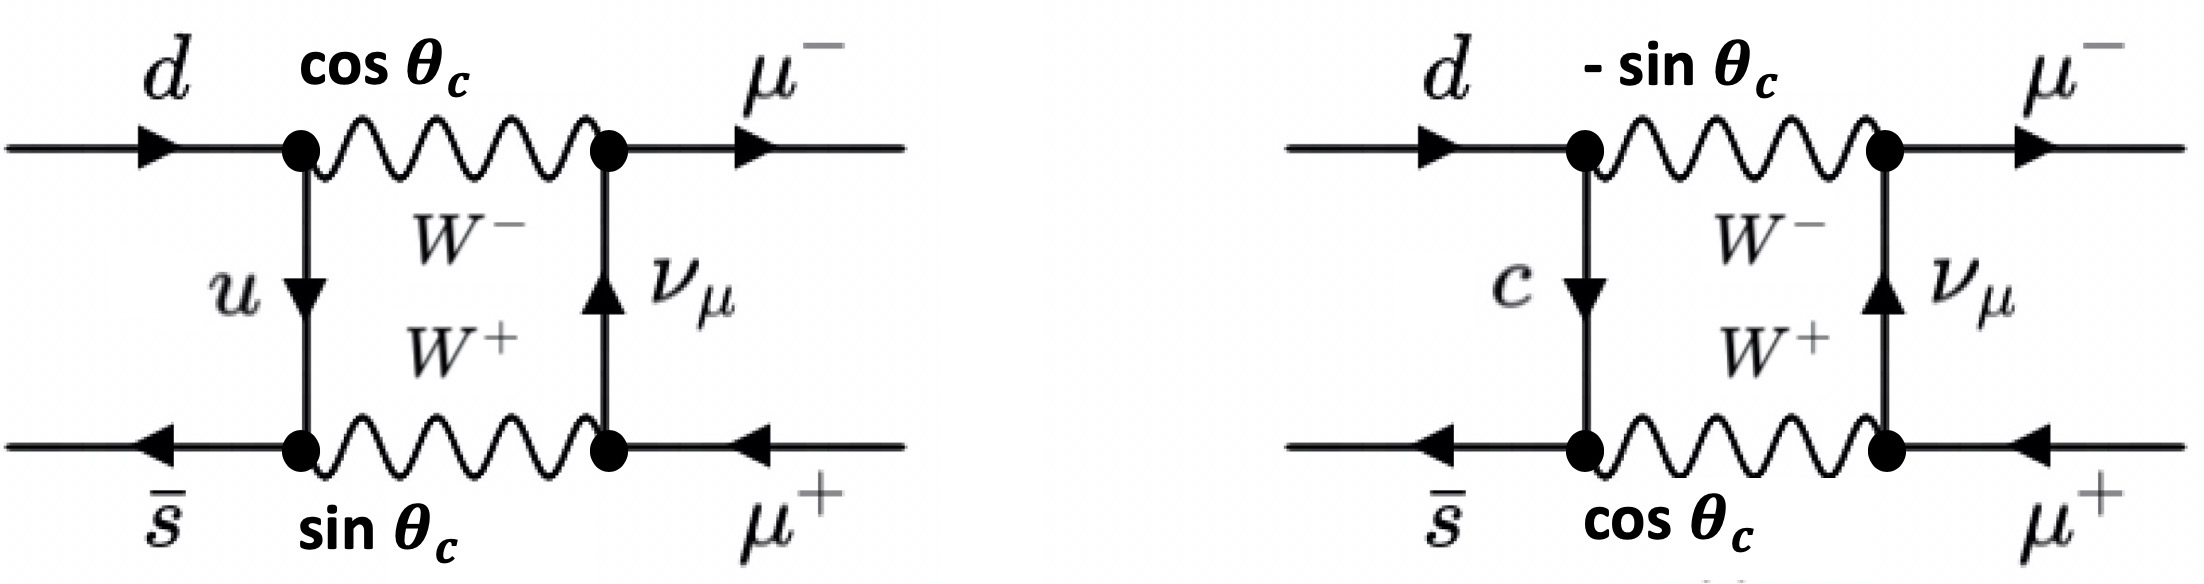
\includegraphics[width=0.8\textwidth]{Chapters/CH1/figures/kdecay}
	\caption{Feynman diagram of $K$ meson decay, a) in CC with BR=,  b) in NC with BR=}
	\label{fig:Kdecay}
\end{figure}
In addition to this major prediction, the GIM mechanism led to the prediction that FCNC processes are forbidden at tree-level Leading Order. The branching ratios of several FCNC decays of the top quark in the SM are given in Table \ref{tab:SM_BR}
\begin{table}[h]
	\begin{adjustbox}{max width=1.\textwidth,center}
		\begin{tabular}{|c|c|c|c|c|c|c|c|c|}
		\hline 
  & $ t\rightarrow uZ$    & $ t\rightarrow cZ$    & $ t\rightarrow u\gamma$ & $ t\rightarrow c\gamma$ & $ t\rightarrow ug$       & $ t\rightarrow cg$       & $ t\rightarrow uH$     & $ t\rightarrow cH$  \\ 
	\hline 
	BR & $8\times 10^{-17} $ & $1\times 10^{-14} $ & $3.7\times 10^{-16} $       & $4.6\times 10^{-14} $      & $3.7\times 10^{-14} $  & $4.6\times 10^{-12} $ & $2\times 10^{-17} $  &$3\times 10^{-15} $  \\ 
		\hline 
		\end{tabular} 
	\end{adjustbox}
\caption{Branching ratios for top quark FCNC interactions in the SM \cite{aguilar}.}
\label{tab:SM_BR}
\end{table}
\noindent The FCNC production is also sensitive to numerous new physics models, as is mentioned in more details in section \ref{sec:bsm}.\\
The GIM hypothesis represent a generalization of Cabibbo's idea. The introduction of the forth quark (c) restored the symmetry
in the (then known)  numbers of quark and leptons.\\
These ideas were extended by Kobayashi and Maskawa (1973), who introduced a framework of six quarks and it will be described in the next section.

\subsubsection{CKM matrix}
In 1973 Kobayashi and Maskawa extended the Cabibbo's mechanism allowing to describe the transitions within and in-between 3 generations of quarks
using the so-called \textit{CKM} $3\times3$ matrix \cite{cabibbo,ckm}, which relates the weak eigenstate of down-type to their mass eigenstate:
\begin{equation}
	\begin{pmatrix}
	d' \\ 
	s' \\ 
	b' 
	\end{pmatrix} 
	= V_{CKM}
	\begin{pmatrix}
	d \\ 
	s \\ 
	b
	\end{pmatrix} 
	=
	\begin{pmatrix}
	|V_ud| & |V_us| & |V_ub| \\ 
	|V_cd| & |V_cs| & |V_cb| \\ 
	|V_td| & |V_ts|  &| V_tb|
	\end{pmatrix} 
	\begin{pmatrix}
	d \\ 
	s \\ 
	b
	\end{pmatrix} 
\end{equation}
By  convention, the up-type quarks are taken to be pure states.
Therefore, partners of the up-type quarks within the weak isospin doublets are the weak eigenstates d’, s’ and b’ which are the pure states. \\
The CKM matrix is fully defined by 4 independent parameters, which must be determined experimentally. These parameters are: 3 mixing angles and 1 CP-mixing
phase, which violates the CP\footnotemark symmetry in the SM \cite{cp_vio}.
The diagonal elements of the CKM matrix are close to 1, reflecting the fact that transitions are favoured between quarks of the same generation. \\
The CKM matrix is unitary, i.e. the sum of the transition probabilities for any quark flavour is equal to 1. If this assumption was to be disproved, 
it could imply the existence of a fourth quark generation \textbf{CITARE FORSE PARAGRAFO BDM}.
\footnotetext{Charge transformation followed by a parity transformation.}

%\clearpage
%\subsection{Electroweak symmetry breaking}  METTERE ???

\clearpage
\section{Top quark physics}

\clearpage
\section{Theories for physics beyond the Standard Model}
\label{sec:bsm}
\clearpage
\subsection{Quark singlets}

\clearpage
\subsection{Two Higgs Doublet Model}

\clearpage
\subsection{Minimal Supersymmetric Standard Model}

\clearpage

